\documentclass[12pt]{report}
\usepackage[spanish]{babel}
\usepackage[utf8]{inputenc}
\usepackage{amsmath}
\usepackage{amssymb}
\usepackage{amsthm}
\usepackage{graphics}
\usepackage{subfigure}
\usepackage{lipsum}
\usepackage{array}
\usepackage{multicol}
\usepackage{enumerate}
\usepackage[framemethod=TikZ]{mdframed}
\usepackage[a4paper, margin = 1.5cm]{geometry}
\usepackage{tikz}
\usepackage{pgffor}
\usepackage{ifthen}
\usepackage{listings}
\usepackage{hyperref}
\usepackage{xcolor}
\usepackage{enumitem}

%Gestión de Hipervínculos

\hypersetup{
    colorlinks=true,
    linkcolor=black,
    filecolor=magenta,      
    urlcolor=cyan
}

%Gestión de Código de Programación

\definecolor{listing-background}{HTML}{F7F7F7}
\definecolor{listing-rule}{HTML}{B3B2B3}
\definecolor{listing-numbers}{HTML}{B3B2B3}
\definecolor{listing-text-color}{HTML}{000000}
\definecolor{listing-keyword}{HTML}{435489}
\definecolor{listing-keyword-2}{HTML}{1284CA} % additional keywords
\definecolor{listing-keyword-3}{HTML}{9137CB} % additional keywords
\definecolor{listing-identifier}{HTML}{435489}
\definecolor{listing-string}{HTML}{00999A}
\definecolor{listing-comment}{HTML}{8E8E8E}

\lstdefinestyle{myStyle}{
    language         = java,
    alsolanguage     = scala,
    numbers          = left,
    xleftmargin      = 2.7em,
    framexleftmargin = 2.5em,
    backgroundcolor  = \color{gray!15},
    basicstyle       = \color{listing-text-color}\linespread{1.0}\ttfamily,
    breaklines       = true,
    frameshape       = {RYR}{Y}{Y}{RYR},
    rulecolor        = \color{black},
    tabsize          = 2,
    numberstyle      = \color{listing-numbers}\linespread{1.0}\small\ttfamily,
    aboveskip        = 1.0em,
    belowskip        = 0.1em,
    abovecaptionskip = 0em,
    belowcaptionskip = 1.0em,
    keywordstyle     = {\color{listing-keyword}\bfseries},
    keywordstyle     = {[2]\color{listing-keyword-2}\bfseries},
    keywordstyle     = {[3]\color{listing-keyword-3}\bfseries\itshape},
    sensitive        = true,
    identifierstyle  = \color{listing-identifier},
    commentstyle     = \color{listing-comment},
    stringstyle      = \color{listing-string},
    showstringspaces = false,
}

\lstset{style = myStyle}

%Gestión de Marca de Agua

\newcounter{it}
\newcommand*\watermarktext[1]{\begin{tabular}{c}
    \setcounter{it}{1}%
    \whiledo{\theit<100}{%
    \foreach \col in {0,...,15}{#1\ \ } \\ \\ \\
    \stepcounter{it}%
    }
    \end{tabular}
    }

\AddToHook{shipout/foreground}{
    \begin{tikzpicture}[remember picture,overlay, every text node part/.style={align=center}]
        \node[rectangle,black,rotate=30,scale=2,opacity=0.04] at (current page.center) {\watermarktext{Cristo Daniel Alvarado ESFM\quad}};
  \end{tikzpicture}
}

%Redefinición de comandos

\def\proof{\paragraph{Demostración:\\}}
\def\endproof{\hfill$\blacksquare$}

\def\sol{\paragraph{Solución:\\}}
\def\endsol{\hfill$\square$}

%Definición de ambientes

\newtheoremstyle{largebreak}
  {}% use the default space above
  {}% use the default space below
  {\normalfont}% body font
  {}% indent (0pt)
  {\bfseries}% header font
  {}% punctuation
  {\newline}% break after header
  {}% header spec

\theoremstyle{largebreak}

\newmdtheoremenv[
    leftmargin=0em,
    rightmargin=0em,
    innertopmargin=0pt,
    innerbottommargin=5pt,
    hidealllines = true,
    roundcorner = 5pt,
    backgroundcolor = gray!60!red!30
]{exa}{Ejemplo}[section]

\newmdtheoremenv[
    leftmargin=0em,
    rightmargin=0em,
    innertopmargin=0pt,
    innerbottommargin=5pt,
    hidealllines = true,
    roundcorner = 5pt,
    backgroundcolor = gray!50!blue!30
]{obs}{Observación}[section]

\newmdtheoremenv[
    leftmargin=0em,
    rightmargin=0em,
    innertopmargin=0pt,
    innerbottommargin=5pt,
    rightline = false,
    leftline = false
]{theor}{Teorema}[section]

\newmdtheoremenv[
    leftmargin=0em,
    rightmargin=0em,
    innertopmargin=0pt,
    innerbottommargin=5pt,
    rightline = false,
    leftline = false
]{propo}{Proposición}[section]

\newmdtheoremenv[
    leftmargin=0em,
    rightmargin=0em,
    innertopmargin=0pt,
    innerbottommargin=5pt,
    rightline = false,
    leftline = false
]{cor}{Corolario}[section]

\newmdtheoremenv[
    leftmargin=0em,
    rightmargin=0em,
    innertopmargin=0pt,
    innerbottommargin=5pt,
    rightline = false,
    leftline = false
]{lema}{Lema}[section]

\newmdtheoremenv[
    leftmargin=0em,
    rightmargin=0em,
    innertopmargin=0pt,
    innerbottommargin=5pt,
    roundcorner=5pt,
    backgroundcolor = gray!30,
    hidealllines = true
]{mydef}{Definición}[section]

\newmdtheoremenv[
    leftmargin=0em,
    rightmargin=0em,
    innertopmargin=0pt,
    innerbottommargin=5pt,
    roundcorner=5pt
]{excer}{Ejercicio}[section]

%Definición de nuevas funciones

\newcommand\abs[1]{\ensuremath{\left|#1\right|}}
\newcommand\divides{\ensuremath{\bigm|}}
\newcommand\cf[3]{\ensuremath{#1:#2\rightarrow#3}}
\newcommand\contradiction{\ensuremath{\#_c}}
\newcommand\natint[1]{\ensuremath{\left[\big|#1\big|\right]}}
\newcommand{\dom}[1]{\textup{dom}\left(#1 \right)}

\begin{document}
    \setlength{\parskip}{5pt} % Añade 5 puntos de espacio entre párrafos
    \setlength{\parindent}{12pt} % Pone la sangría como me gusta
    \title{Curso de Lógica Matemática
    
    Teoría de la Computabilidad}
    \author{Cristo Daniel Alvarado}
    \maketitle

    \tableofcontents %Con este comando se genera el índice general del libro

    \newpage

    \setcounter{chapter}{2}

    \chapter{Conjuntos y Funciones computables}

    Todo de lo que se va a tratar esta parte es de: ¿Cómo formalizar la noción de \textit{procedimiento mecánico, efectivo} o \textit{sistemático}? Con esto nos referimos a:
    \begin{itemize}
        \item Tener un número finito de instrucciones.
        \item Terminar el procedimiento en un número finito de pasos.
        \item Usar únicamente \textit{papel y lápiz}.
        \item No requiere razonamiento, solo se siguen reglas.
    \end{itemize}

    Básicamente se pretendía que dada una fórmula, encontrar un algoritmo que nos diga si esa fórmula es verdadera o falsa. Básicamente se pretendía formalizar las demostraciones para ver lo que nosotros podemos demostrar únicamente usando los axiomas.

    Turing y Alonzo Church eventualmente se hicieron preguntas en la misma dirección. En la Tesis de Church-Turing se probó que estas tres preguntas en realidad se reducen a un mismo problema.

    \section{Máquinas de Turing}

    \begin{mydef}
        Una \textbf{máquina de Turing} consta de:
        \begin{itemize}
            \item Un \textit{alfabeto}, un conjunto finito $L$.
            \item Un conjunto $S$ de \textit{estados}.
            \item Una función parcial $\cf{T}{L^*\times S}{L^*\times S\times\left\{<,-,> \right\}}$ llamada \textit{función de transición}.
        \end{itemize}
        donde $L^*=L\cup\left\{* \right\}$.
    \end{mydef}

    Intuitivamente, uno debe imaginar que esto es una especie de \textit{computadora rudimentaria}. Generalmente esto se conceptualiza como una cinta.

    \begin{center}
        \label{Turing1}
        \begin{figure}
            \begin{center}
                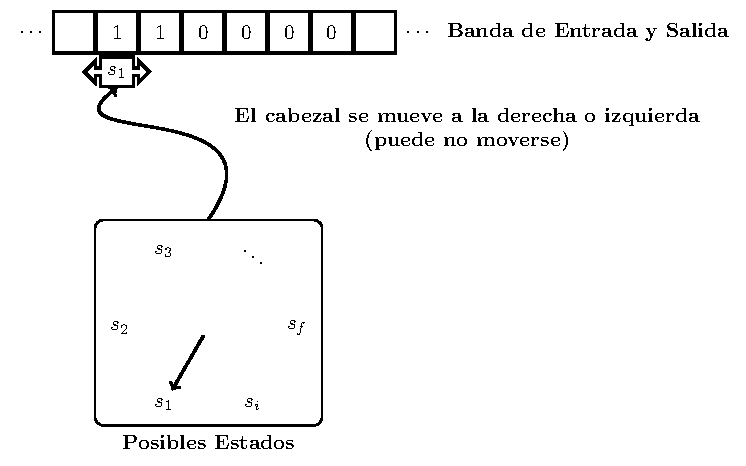
\includegraphics[scale=1]{images/fig_1.pdf}
            \end{center}
            \caption{Ejemplo de Máquina de Turing}
        \end{figure}
    \end{center}

   El cabezal $c$ puede moverse a la derecha, izquierda o no moverse, dependiendo del estado en el que esté. En la Figura \ref{Turing1} se muestra que el hay al menos 5 diferentes estados, desde el estado inicial ($s_i$) hasta el final ($s_f$). Dependiendo de la entrada, la función $T$ nos dirá lo que hará el cabezal, si cambia un elemento de la banda, si se mueve o si cambia de estado (o todas a la vez).

   En este ejemplo, el alfabeto sería $L=\left\{0,1 \right\}$, el conjunto de estados es $S=\left\{s_i,s_1,...,s_f \right\}$ y la función sería representada por lo que sea que haga el cabezal.

    \begin{exa}
        Considere $L=\left\{1 \right\}$, $S=\left\{s_i,s_1,s_2 \right\}$ y,
        \begin{equation*}
            T=\left\{(s_i,*,s_1,*,>),(s_i,1,s_1,1,>),(s_1,1,s_1,1,>),(s_1,1,s_2,1,-) \right\}
        \end{equation*}
        La cinta se ve más o menos así:

    \end{exa}

    Para los siguientes ejercicios, ir a la página: \href{https://turingmachinesimulator.com/}{Simulador Máquina de Turing}.

    \begin{excer}
        Codifique una máquina de Turing que sume 1 a un número dado en binario.
    \end{excer}

    \begin{lstlisting}
        name: Sumar uno en unario
        init: s0
        accept: sf

        
        // Funciones de Transicion

        s0,_
        s0,_,>

        s0,1
        s1,1,-

        s0,0
        s1,0,-

        s1,1
        s1,0,>

        s1,0
        s1,1,>

        s1,_
        sf,_,-

        // < = left
        // > = right
        // - = hold
        // use _ for blank cells

        // States and symbols are case-sensitive

        // Load your code and click COMPILE.
        //  or load an example (top-right).
    \end{lstlisting}

    \begin{excer}
        Codifique una máquina de Turing que dada un número en binario, invierta su orientación, es decir, si la cadena es $(a_1,...,a_n)$, que la máquina de Turing la convierta en $(a_n,...,a_1)$. 
    \end{excer}

    \begin{lstlisting}
        name: invertirCadena
        init: s0
        accept: s1,sf,l,c,u
        
        //esto para que se empiece a mover
        s0,_
        s0,_,>
        
        s0,0
        x,0,<
        
        s0,1
        x,1,<
        
        x,_
        s1,2,>
        
        s1,0
        s1,0,>
        
        s1,1
        s1,1,>
        
        //logica cuando encuentre cosas
        
        s1,_
        s2,_,<
        
        s2,_
        s2,_,<
        
        s2,0
        c00,_,>
        
        s2,1
        u00,_,>
        
        //mueve cosas al inicio
        
        c00,_
        m,0,<
        
        u00,_
        m,1,<
        
        //ya en ciclo
        
        //mueve derecha
        
        m,_
        l,_,<
        
        l,_
        l,_,<
        
        l,0
        c0,_,>
        
        l,1
        u0,_,>
        
        c0,_
        c0,_,>
        
        //mueve izquierda
        
        u0,_
        u0,_,>
        
        c0,0
        c1,0,>
        
        c0,1
        c1,1,>
        
        u0,0
        u1,0,>
        
        u0,1
        u1,1,>
        
        c1,0
        c1,0,>
        
        c1,1
        c1,1,>
        
        u1,0
        u1,0,>
        
        u1,1
        u1,1,>
        
        c1,_
        m,0,<
        
        u1,_
        m,1,<
        
        m,0
        m,0,<
        
        m,1
        m,1,<
        
        l,2
        sf,_,>
        
        sf,_
        sf,_,>
        
        sf,0
        sff,0,-
        
        sf,1
        sff,1,-        
    \end{lstlisting}

    \begin{mydef}
        Una función $f$ es \textbf{computable} si:
        \begin{enumerate}[label = \textit{(\arabic*)}]
            \item $\dom{f}\subseteq\mathbb{N}$.
            \item Existe un algoritmo tal que para cada $n\in\mathbb{N}$, el algoritmo al correrse con $n$ como argumento, se detiene en tiempo finito si y sólo si $n\in\dom{f}$ y en tal caso arroja $f(n)$ como salida. 
        \end{enumerate}
    \end{mydef}

    ¿Qué es un algoritmo? Resulta que hay muchas formas de definirlo, sin embargo, nosotros adoptaremos la siguiente definición:

    \begin{mydef}
        Un \textbf{algoritmo} lo interpretaremos como una máquina de Turing.
    \end{mydef}

    \begin{obs}
        Un algoritmo también puede verse como un código en C, C++, Python o \LaTeX (usando las librerías adecuadas).
    \end{obs}

    En la Tesis de Church-Turing, cualquier noción es equivalente.

    \begin{obs}
        De ahora en adelante consideraremos a los naturales con el 0.
    \end{obs}

    \begin{exa}
        La función $\cf{f}{\mathbb{N}\setminus\left\{0,1\right\}}{\mathbb{N}}$ tal que $n\mapsto\min\left\{p\in\mathbb{N}\Big|p\textup{ es primo y }p\divides n \right\}$ es computable.
    \end{exa}

    \begin{proof}
        Se tiene el siguiente algoritmo:
        \begin{lstlisting}
int f(int n){
    for(int k = 2;n % k != 0;k++) return k;
}
        \end{lstlisting}
    \end{proof}

    \begin{exa}
        Considere la función $\cf{g}{\left\{n^2\Big|n\in\mathbb{N} \right\}}{\mathbb{N}}$ dada por $n^2\mapsto n$. Esta función es computable.
    \end{exa}

    \begin{proof}
        Se tiene el siguiente algoritmo:
        \begin{lstlisting}
int g(int m){
    for(int k = 0;k*k != m;k++) return k;
}
        \end{lstlisting}
    \end{proof}

    \begin{exa}
        La función $\cf{+}{\mathbb{N}\times\mathbb{N}}{\mathbb{N}}$ es computable.
    \end{exa}

    \begin{proof}
        Recordemos que existe una biyección entre $\mathbb{N}\times\mathbb{N}$ y $\mathbb{N}$ dada por:
        \begin{equation*}
            (k,l)\mapsto 2^k(2l+1)
        \end{equation*}
        por lo cual, podemos ver a la función suma como una función de $\mathbb{N}$ en $\mathbb{N}$.
    \end{proof}

    \begin{obs}
        Podemos ir más allá en el ejemplo anterior, podemos generalizar la idea anterior usando conjuntos que puedan ser representados mediante números naturales (recuerde la enumeración de Gödel).
    \end{obs}

    Veremos más ejemplos que nos ayudarán más adelante a hacer cosas más complejas:

    \begin{itemize}
        \item La función sucesor (se vió en un ejercicio anterior).
        \item Cualquier función constante.
        \item La $i$-ésima proyección de una $k$-tupla.
    \end{itemize}
    \begin{lstlisting}
int p_2(int a, int b, int c){
    return b;
}
    \end{lstlisting}
    este ejemplo anterior es la 2-ésima proyección de una 3-tupla.

    \begin{exa}
        La función exponencial: $(a,b)\mapsto a^{b}$ es computable.
    \end{exa}

    \begin{proof}
        En efecto, se tiene el siguiente algoritmo:
        \begin{lstlisting}
int exp(int a, int b){
    if(b==0){
        return 1;
    }
    else return a*exp(a,b-1);
}
        \end{lstlisting}
    \end{proof}

    \begin{exa}
        La función factorial $n\mapsto n!$ es computable.
    \end{exa}

    \begin{proof}
        En efecto, se tiene el siguiente algoritmo:
        \begin{lstlisting}
int fact(int n){
    if(n==0) return 1;
    else return n*fact(n-1);
}
        \end{lstlisting}
    \end{proof}

    \begin{exa}
        Las funciones máximo y mínimo son computables.
    \end{exa}

    \begin{exa}
        El algoritmo de la división es computable.
    \end{exa}

    \begin{proof}
        En efecto, se tiene el siguiente algoritmo:
        \begin{lstlisting}
int div(int a, int b){
    for(int i=1; i*b<=a;i++){} //se queda y acaba si es que se puede dividir
    q = i-1;
    r = a-b*q;
    return exp(2,q)*(2*r-1); //codificamos de esta manera la salida del programa
}
        \end{lstlisting}
    \end{proof}

    \begin{obs}
        Cuando coloquemos $\cf{f}{;A}{B}$, entenderemos que $\dom{f}\subseteq A$, es decir que $f$ es una función parcial.
    \end{obs}

    \begin{theor}
        Sea $\cf{f}{;\mathbb{N}^k}{\mathbb{N}}$ una función computable, y sean $\cf{g_1,...,g_k}{;\mathbb{N}}{\mathbb{N}}$ funciones computables. Entonces:
        \begin{enumerate}[label = \textit{(\arabic*)}]
            \item La función $\cf{h_1}{;\mathbb{N}}{\mathbb{N}}$ dada por: $h_1(x)=f(g_1(x),\cdots,g_k(x))$ es computable.
            \item La función $\cf{h_2}{;\mathbb{N}^{ k-1}}{\mathbb{N}}$ dada por:
            \begin{equation*}
                h_2(x_2,\cdots,x_k)=(\mu x)(f(x,x_2,\cdots,x_k)=0)
            \end{equation*}
            donde la función $\mu x$ es el mínimo de $x$ tal que lo de adentro se hace 0, siendo $f$ tal que para todo $i\leq x$, $f(i,x_2,...,x_k)$ está bien definido, también es computable.
        \end{enumerate}
    \end{theor}

    \begin{proof}
        De \textit{(1)}: Considere el algoritmo:
        \begin{lstlisting}
int h_1(int x){
    int y_1 = g_1(x);
    int y_2 = g_2(x);
    ...
    int y_k = g_k(x);
    return f(y_1,...,y_k);
}
        \end{lstlisting}
    \end{proof}
    es una función computable, ya que si no puede calcular algún valor, se queda atorado.

    De \textit{(2)}: Considere el algoritmo:
    \begin{lstlisting}
        int h_2(int x_2,...,int x_k){
            for(int x=0; f(x,x_2,...,x_k)!=0;x++) return x;
        }
    \end{lstlisting}
    es de una función computable.

    \begin{mydef}
        Una función computable $\cf{f}{;\mathbb{N}^k}{\mathbb{N}}$ es \textbf{total}, si $\dom{f}=\mathbb{N}^k$. En computabilidad esto se denota por:
        \begin{equation*}
            (\forall x_1,...,x_k)(f(x_1,...,x_k)\downarrow)
        \end{equation*}
        esto es, que para cualquier entrada $f$ está bien definida.
    \end{mydef}

    \begin{obs}
        En el teorema anterior, siempre se puede hacer (2) si la función $f$ es total.
    \end{obs}




    

    \chapter{Teoremas de Completud}


\end{document}